\documentclass[11pt,a4paper]{article}
\usepackage[utf8]{vietnam}
\usepackage{mathptmx} % Times New Roman
\usepackage[left=2cm,right=2cm,top=2cm,bottom=2cm,headheight=15pt]{geometry}
\usepackage{amsmath,amssymb,amsfonts}
\usepackage{xcolor}
\usepackage{graphicx}
\usepackage{booktabs}
\usepackage{tabularx}
\usepackage{array}
\usepackage{enumitem}
\usepackage{fancyhdr}
\usepackage{lastpage}
\usepackage{tasks}

% Thiết lập tasks cho trắc nghiệm
\settasks{label=\textbf{\Alph*.}, label-width=1.5em, item-indent=2.5em, column-sep=1em}

% Định nghĩa khối đáp án và hướng dẫn giải ở từng câu
\newcommand{\giaithich}[2]{%
    \par\vspace{0.15cm}\noindent
    \begingroup\small
    \noindent\textbf{\color{blue}$\blacktriangleright$ Đáp án đúng: #1} \par\vspace{0.08cm}
    \noindent\textbf{\color{teal}$\blacktriangleright$ Hướng dẫn giải:} #2
    \endgroup\par\vspace{0.35cm}
}

% Thiết lập header & footer
\pagestyle{fancy}
\fancyhf{}
\lfoot{Mã đề: 001}
\rfoot{Trang \thepage/\pageref{LastPage}}
\renewcommand{\headrulewidth}{0pt}
\renewcommand{\footrulewidth}{0.4pt}

\begin{document}

% --- TIÊU ĐỀ ĐỀ THI ---
\noindent
\begin{minipage}[t]{0.48\textwidth}
    \centering
    \textbf{TRƯỜNG ĐẠI HỌC CÔNG NGHỆ THÔNG TIN}\\
    \textbf{TRUNG TÂM PHÁT TRIỂN}\\
    \textbf{CÔNG NGHỆ THÔNG TIN}\\
    \vspace{0.2cm}
    \textbf{Đề: 001}
\end{minipage}
\hfill
\begin{minipage}[t]{0.48\textwidth}
    \centering
    \textbf{ĐỀ THI CUỐI HỌC KỲ: I (2024-2025)}\\
    \textbf{MÔN: HỆ ĐIỀU HÀNH}\\
    \textbf{Hệ: Đào tạo từ xa}\\
    \vspace{0.2cm}
    \textit{Thời gian: 75 phút}
\end{minipage}

\vspace{0.3cm}
\begin{center}
    \textit{(Sinh viên không được sử dụng tài liệu. Làm bài trực tiếp trên đề)}
\end{center}

\vspace{0.2cm}

% --- BẢNG THÔNG TIN SINH VIÊN VÀ ĐIỂM ---
\noindent
\begin{tabularx}{\textwidth}{|X|p{2.2cm}|p{4cm}|}
\hline
\textbf{HỌ VÀ TÊN SV:} \dotfill & \centering\textbf{ĐIỂM} & \centering\textbf{CÁN BỘ COI THI} \tabularnewline
\textbf{MSSV:} \dotfill & & \tabularnewline
\textbf{STT:} \dotfill & & \tabularnewline
\textbf{PHÒNG THI:} \dotfill & & \tabularnewline
\hline
\end{tabularx}

\vspace{0.4cm}

% --- BẢNG TRẢ LỜI TRẮC NGHIỆM ---
\begin{center}
    \textbf{\large BẢNG TRẢ LỜI TRẮC NGHIỆM}
\end{center}

\vspace{0.1cm}
\noindent
\begin{tabularx}{\textwidth}{|*{7}{>{\centering\arraybackslash}X|}}
\hline
\textbf{Câu 1} & \textbf{Câu 2} & \textbf{Câu 3} & \textbf{Câu 4} & \textbf{Câu 5} & \textbf{Câu 6} & \textbf{Câu 7} \\ \hline
\textbf{\color{blue}A} & \textbf{\color{blue}A} & \textbf{\color{blue}C} & \textbf{\color{blue}C} & \textbf{\color{blue}D} & \textbf{\color{blue}D} & \textbf{\color{blue}C} \\ \hline
\textbf{Câu 8} & \textbf{Câu 9} & \textbf{Câu 10} & \textbf{Câu 11} & \textbf{Câu 12} & \textbf{Câu 13} & \textbf{Câu 14} \\ \hline
\textbf{\color{blue}A} & \textbf{\color{blue}D} & \textbf{\color{blue}B} & \textbf{\color{blue}D} & \textbf{\color{blue}B} & \textbf{\color{blue}C} & \textbf{\color{blue}A} \\ \hline
\textbf{Câu 15} & \textbf{Câu 16} & \textbf{Câu 17} & \textbf{Câu 18} & \textbf{Câu 19} & \textbf{Câu 20} & \textbf{Câu 21} \\ \hline
\textbf{\color{blue}C} & \textbf{\color{blue}C} & \textbf{\color{blue}A} & \textbf{\color{blue}B} & \textbf{\color{blue}A} & \textbf{\color{blue}D} & \textbf{\color{blue}D} \\ \hline
\textbf{Câu 22} & \textbf{Câu 23} & \textbf{Câu 24} & \textbf{Câu 25} & \textbf{Câu 26} & \textbf{Câu 27} & \textbf{Câu 28} \\ \hline
\textbf{\color{blue}C} & \textbf{\color{blue}B} & \textbf{\color{blue}D} & \textbf{\color{blue}B} & \textbf{\color{blue}A} & \textbf{\color{blue}B} & \textbf{\color{blue}B} \\ \hline
\end{tabularx}

\vspace{0.4cm}

% --- BẢNG TRẢ LỜI TỰ LUẬN ---
\begin{center}
    \textbf{\large BẢNG TRẢ LỜI TỰ LUẬN}
\end{center}

\vspace{0.1cm}
\noindent
\begin{tabularx}{\textwidth}{|*{4}{>{\centering\arraybackslash}X|}}
\hline
\textbf{Câu 29} & \textbf{Câu 30} & \textbf{Câu 31} & \textbf{Câu 32} \\ \hline
\textbf{\color{blue}70} & \textbf{\color{blue}RAG} & \textbf{\color{blue}Waiting} & \textbf{\color{blue}$2^{20}$} \\ \hline
\end{tabularx}

\newpage

% --- NỘI DUNG ĐỀ THI ---
\noindent\textbf{\large PHẦN 1: TRẮC NGHIỆM}\\
\textit{(07 điểm, 0.25 điểm/câu, SV chọn 1 đáp án đúng nhất và điền vào BẢNG TRẢ LỜI TRẮC NGHIỆM)}

\vspace{0.3cm}
\noindent\textit{Sử dụng dữ liệu sau để trả lời câu 1, 2, 3:}\\
Giả sử một tiến trình được cấp 4 khung trang trong bộ nhớ vật lý và 7 trang trong bộ nhớ ảo. Tại thời điểm nạp tiến trình vào, 4 khung trang trên bộ nhớ vật lý này đang trống. Tiến trình truy xuất 7 trang (1, 2, 3, 4, 5, 6, 7) trong bộ nhớ ảo theo thứ tự như sau:
\[ 4\quad 2\quad 4\quad 4\quad 5\quad 7\quad 3\quad 1\quad 4\quad 2\quad 1\quad 7\quad 5\quad 6\quad 5\quad 2\quad 4\quad 3\quad 5\quad 1 \]

\noindent\textbf{Câu 1:} Tại thời điểm tiến trình truy xuất trang nhớ số 7 lần đầu tiên, trang nhớ nào sẽ bị thay thế, nếu sử dụng giải thuật thay thế trang FIFO?
\begin{tasks}(2)
    \task Không trang nhớ nào bị thay thế
    \task 2
    \task 5
    \task 4
\end{tasks}
\giaithich{A}{Tại thời điểm truy xuất trang 7 lần đầu tiên (bước thứ 6 trong chuỗi: 4, 2, 4, 4, 5, 7), các khung trang vật lý trước đó mới chỉ nạp các trang \{4, 2, 5\} (mới sử dụng 3 khung trang). Khung trang thứ 4 vẫn đang trống, do đó trang 7 được nạp trực tiếp vào khung trang còn trống này mà không cần thay thế bất kỳ trang nào.}

\noindent\textbf{Câu 2:} Tại thời điểm tiến trình truy xuất trang nhớ số 6 lần đầu tiên, có tổng cộng bao nhiêu lỗi trang đã xảy ra nếu sử dụng giải thuật thay thế trang OPT (không tính lỗi trang khi truy xuất trang 6)?
\begin{tasks}(4)
    \task 7
    \task 8
    \task 9
    \task 6
\end{tasks}
\giaithich{A}{Mô phỏng giải thuật OPT (Optimal) với 4 khung trang cho đến trước bước 14 (truy xuất trang 6):
\begin{itemize}[noitemsep,topsep=1pt]
    \item Bước 1 (trang 4): Nạp vào khung $\rightarrow$ [4] (Lỗi trang 1)
    \item Bước 2 (trang 2): Nạp vào khung $\rightarrow$ [4, 2] (Lỗi trang 2)
    \item Bước 3, 4 (trang 4): Đã có trong bộ nhớ $\rightarrow$ Hit
    \item Bước 5 (trang 5): Nạp vào khung $\rightarrow$ [4, 2, 5] (Lỗi trang 3)
    \item Bước 6 (trang 7): Nạp vào khung $\rightarrow$ [4, 2, 5, 7] (Lỗi trang 4)
    \item Bước 7 (trang 3): Bộ nhớ đầy. Xét các trang tương lai (1, 4, 2, 1, 7, 5, 6...), trang 5 được dùng xa nhất $\rightarrow$ Thay trang 5 $\rightarrow$ [4, 2, 3, 7] (Lỗi trang 5)
    \item Bước 8 (trang 1): Xét tương lai (4, 2, 1, 7, 5, 6...), trang 3 dùng xa nhất $\rightarrow$ Thay trang 3 $\rightarrow$ [4, 2, 1, 7] (Lỗi trang 6)
    \item Bước 9 (trang 4), Bước 10 (trang 2), Bước 11 (trang 1), Bước 12 (trang 7): Đều có sẵn trong khung $\rightarrow$ Hit
    \item Bước 13 (trang 5): Xét tương lai (6, 5, 2, 4, 3, 5, 1), trang 7 không còn xuất hiện $\rightarrow$ Thay trang 7 $\rightarrow$ [4, 2, 1, 5] (Lỗi trang 7)
\end{itemize}
Như vậy, trước khi truy xuất trang 6 ở bước 14, có đúng 7 lỗi trang đã xảy ra.}

\noindent\textbf{Câu 3:} Nếu sử dụng giải thuật LRU, có tổng cộng bao nhiêu lỗi trang xảy ra?
\begin{tasks}(4)
    \task 12
    \task 10
    \task 15
    \task 8
\end{tasks}
\giaithich{C}{Mô phỏng giải thuật LRU (Least Recently Used) cho toàn bộ chuỗi 20 truy xuất:
Các lỗi trang phát sinh lần lượt ở: Bước 1 (nạp 4), Bước 2 (nạp 2), Bước 5 (nạp 5), Bước 6 (nạp 7), Bước 7 (nạp 3 thay 4), Bước 8 (nạp 1 thay 2), Bước 9 (nạp 4 thay 5), Bước 10 (nạp 2 thay 7), Bước 12 (nạp 7 thay 3), Bước 13 (nạp 5 thay 4), Bước 14 (nạp 6 thay 2), Bước 16 (nạp 2 thay 7), Bước 17 (nạp 4 thay 1), Bước 18 (nạp 3 thay 6), Bước 20 (nạp 1 thay 2). Tổng cộng xảy ra đúng 15 lỗi trang.}

\noindent\textbf{Câu 4:} Một bộ vi xử lý có không gian địa chỉ ảo 32 bit. Hỏi bảng trang có bao nhiêu mục (entry) nếu kích thước bảng trang là 512KB và kích thước của mỗi mục là 4 bytes?
\begin{tasks}(4)
    \task $2^{19}$
    \task $2^{16}$
    \task $2^{17}$
    \task $2^{18}$
\end{tasks}
\giaithich{C}{Số lượng mục (entries) trong bảng trang được tính trực tiếp từ dung lượng bảng trang chia cho kích thước một mục:
$$\text{Số mục} = \frac{\text{Kích thước bảng trang}}{\text{Kích thước mỗi mục}} = \frac{512\text{ KB}}{4\text{ Bytes}} = \frac{512 \times 2^{10}}{4} = 128 \times 2^{10} = 2^7 \times 2^{10} = 2^{17}\text{ mục.}$$}

\noindent\textbf{Câu 5:} Trong mô hình quản lý bộ nhớ, tiến trình có thể chuyển đổi địa chỉ tại các thời điểm nào sau đây?
\begin{tasks}(2)
    \task Thời điểm nạp
    \task Thời điểm thực thi
    \task Thời điểm biên dịch
    \task Tất cả đáp án đều đúng
\end{tasks}
\giaithich{D}{Theo giáo trình Quản lý bộ nhớ (Chương 7), sự liên kết địa chỉ (Address Binding) và chuyển đổi địa chỉ từ logic sang vật lý có thể diễn ra tại một trong 3 thời điểm:
1. Thời điểm biên dịch (Compile time) nếu biết trước vị trí bộ nhớ;
2. Thời điểm nạp (Load time) nếu vị trí chưa biết lúc biên dịch;
3. Thời điểm thực thi (Execution/Run time) nếu tiến trình có thể di chuyển trong bộ nhớ trong lúc chạy. Do đó, cả 3 phương án đều đúng.}

\noindent\textbf{Câu 6:} Hình bên dưới mô tả việc ứng dụng semaphore để đảm bảo thao tác S1 trong P1 luôn thực thi trước thao tác S2 trong P2, biết synch là một semaphore, hãy cho biết giá trị của synch cần được khởi tạo là bao nhiêu?
\begin{center}
    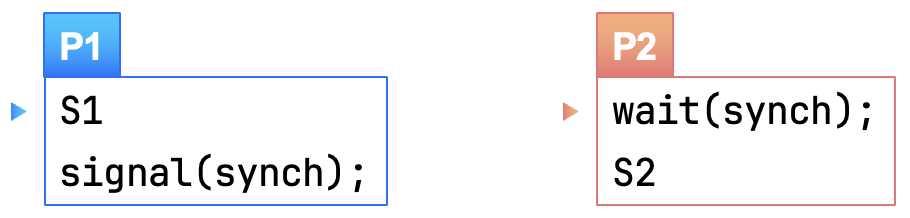
\includegraphics[width=0.48\textwidth]{images/synch_cau20.png}
\end{center}
\begin{tasks}(4)
    \task 1
    \task -1
    \task 2
    \task 0
\end{tasks}
\giaithich{D}{Để ép buộc thứ tự thực thi $S_1$ xong trước rồi mới đến $S_2$:
Tiến trình $P_1$ chạy xong $S_1$ thì gọi \texttt{signal(synch)}; Tiến trình $P_2$ muốn chạy $S_2$ thì trước tiên phải gọi \texttt{wait(synch)}.
Để đảm bảo nếu $P_2$ tới trước khi $P_1$ chạy xong $S_1$ thì $P_2$ phải bị chặn (block), biến Semaphore \texttt{synch} bắt buộc phải được khởi tạo giá trị ban đầu bằng \textbf{0}.}

\noindent\textbf{Câu 7:} Xét một hệ thống sử dụng kỹ thuật phân trang với bảng trang được lưu trữ trong bộ nhớ chính. Nếu thời gian tìm kiếm trong TLB là $\varepsilon = 25\text{ns}$, thời gian một chu kỳ truy xuất bộ nhớ ($x$) là 200ns, và thời gian truy xuất bộ nhớ hiệu dụng (EAT) là 250ns. Hỏi tỉ lệ tìm thấy trang nhớ trong TLB ($\alpha$) là bao nhiêu?
\begin{tasks}(4)
    \task 90.7\%
    \task 85.7\%
    \task 87.5\%
    \task 95.0\%
\end{tasks}
\giaithich{C}{Công thức tính thời gian truy xuất bộ nhớ hiệu dụng có TLB:
$$\text{EAT} = \varepsilon + \alpha \times m + (1 - \alpha) \times 2m = \varepsilon + 2m - \alpha \times m$$
Thay các giá trị: $\text{EAT} = 250\text{ ns}$, $\varepsilon = 25\text{ ns}$, $m = 200\text{ ns}$:
$$250 = 25 + 2 \times 200 - \alpha \times 200 = 425 - 200\alpha$$
$$200\alpha = 425 - 250 = 175 \implies \alpha = \frac{175}{200} = 0.875 = 87.5\%.$$}

\noindent\textbf{Câu 8:} Trong các giải thuật thay thế trang, giải thuật nào yêu cầu thêm sự hỗ trợ từ phần cứng để thực hiện?
\begin{tasks}(1)
    \task LRU
    \task OPT
    \task Không có giải thuật nào yêu cầu thêm sự hỗ trợ từ phần cứng
    \task FIFO
\end{tasks}
\giaithich{A}{Giải thuật LRU (Least Recently Used) cần xác định chính xác trang nào ít được dùng nhất gần đây. Điều này đòi hỏi phần cứng phải cung cấp cơ chế ghi nhận thời gian hoặc thứ tự truy xuất, cụ thể là bằng Bộ đếm (Counter/Clock) hoặc Ngăn xếp (Stack) cập nhật tại mỗi chu kỳ truy xuất bộ nhớ.}

\noindent\textbf{Câu 9:} Biết rằng trong hình bên dưới, các semaphore S và Q được khởi tạo với giá trị là 1. Hãy cho biết vấn đề có thể xảy ra khi P1 và P2 thực thi đồng thời với nhau?
\begin{center}
    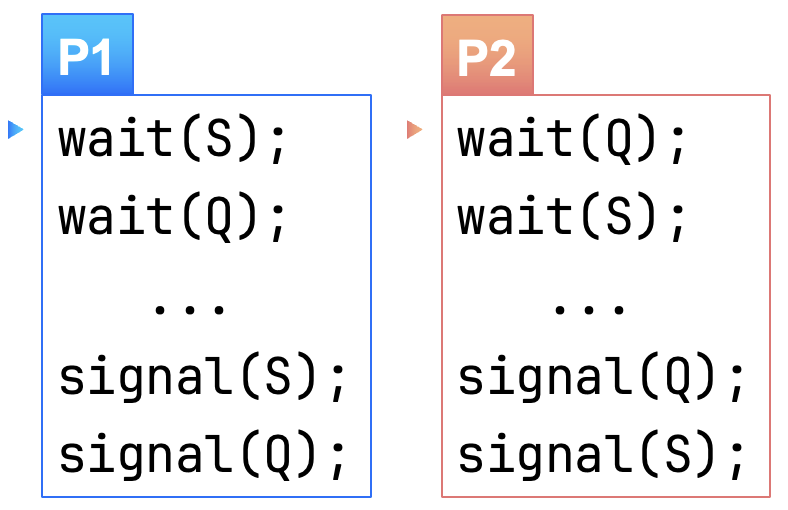
\includegraphics[width=0.38\textwidth]{images/deadlock_cau9.png}
\end{center}
\begin{tasks}(1)
    \task Không có vấn đề gì xảy ra
    \task Tiến trình P2 luôn thực thi trước tiến trình P1
    \task Tiến trình P1 luôn thực thi trước tiến trình P2
    \task P1 và P2 có thể bị deadlock
\end{tasks}
\giaithich{D}{Quan sát mã nguồn:
Tiến trình $P_1$ gọi \texttt{wait(S)} rồi mới gọi \texttt{wait(Q)}; trong khi tiến trình $P_2$ gọi ngược lại: \texttt{wait(Q)} rồi mới gọi \texttt{wait(S)}.
Nếu $P_1$ thực hiện xong \texttt{wait(S)} (chiếm $S$) đồng thời $P_2$ thực hiện xong \texttt{wait(Q)} (chiếm $Q$), thì sau đó $P_1$ sẽ bị khóa khi chờ $Q$, còn $P_2$ bị khóa khi chờ $S$. Cả hai tiến trình vĩnh viễn không thể tiếp tục, dẫn đến \textbf{Tắc nghẽn (Deadlock)}.}

\noindent\textbf{Câu 10:} Để áp dụng giải thuật Banker, tiến trình cần phải khai báo những thông tin gì?
\begin{tasks}(1)
    \task Số lượng thực thể tối thiểu mà tiến trình cần ở mỗi loại tài nguyên
    \task Số lượng thực thể tối đa của mỗi loại tài nguyên mà tiến trình cần
    \task Số lượng tài nguyên tối đa mà tiến trình cần
    \task Dung lượng bộ nhớ tối đa mà tiến trình cần
\end{tasks}
\giaithich{B}{Giải thuật Banker (thuộc nhóm giải thuật tránh deadlock của Dijkstra) yêu cầu tiên quyết là mỗi tiến trình khi gia nhập hệ thống phải khai báo trước ma trận \textbf{Max}, tức là số lượng thực thể tối đa của từng loại tài nguyên mà tiến trình có thể yêu cầu trong suốt quá trình hoạt động.}

\noindent\textbf{Câu 11:} Cho 4 đồ thị cấp phát tài nguyên (a), (b), (c), (d) như hình bên dưới trong đó T1, T2, T3, T4 là các tiến trình và R1, R2, R3 là các tài nguyên. Hỏi đồ thị nào có deadlock xảy ra?
\begin{center}
    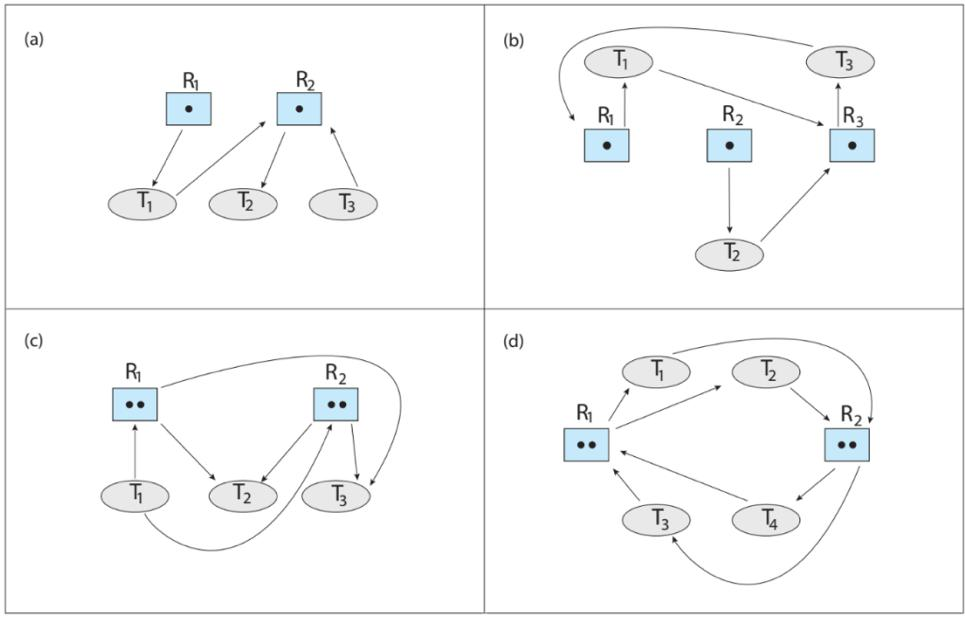
\includegraphics[width=0.68\textwidth]{images/rag_cau11.png}
\end{center}
\begin{tasks}(2)
    \task Đồ thị (a), (b)
    \task Đồ thị (c), (d)
    \task Đồ thị (b), (c), (d)
    \task Đồ thị (b), (d)
\end{tasks}
\giaithich{D}{Phân tích đồ thị cấp phát tài nguyên (RAG):
\begin{itemize}[noitemsep,topsep=1pt]
    \item Đồ thị (b): Có một chu trình đơn thực thể $T_1 \to R_1 \to T_2 \to R_2 \to T_1$. Vì mỗi tài nguyên chỉ có đúng 1 thực thể nên chu trình này chắc chắn gây ra \textbf{Deadlock}.
    \item Đồ thị (d): Tồn tại chu trình khóa chéo giữa cả 4 tiến trình và tất cả các thực thể tài nguyên đều bị chiếm giữ bởi các tiến trình trong chu trình $\rightarrow$ \textbf{Deadlock}.
    \item Đồ thị (a) và (c): Các tài nguyên có nhiều thực thể và tồn tại các tiến trình ngoài chu trình có thể hoàn thành rồi giải phóng tài nguyên để phá vỡ chu trình $\rightarrow$ Không bị deadlock.
\end{itemize}
Vậy đồ thị có deadlock là \textbf{(b) và (d)}.}

\noindent\textbf{Câu 12:} Nghịch lý Belady là gì?
\begin{tasks}(1)
    \task Hiện tượng số lỗi trang giảm khi tiến trình được cấp nhiều frame hơn
    \task Hiện tượng số lỗi trang tăng mặc dù tiến trình được cấp nhiều frame hơn
    \task Hiện số lỗi trang tăng mặc dù tiến trình được cấp ít frame lại
    \task Hiện tượng số lỗi trang không đổi khi tiến trình được cấp nhiều frame hơn
\end{tasks}
\giaithich{B}{Nghịch lý Belady (Belady's Anomaly) là hiện tượng ngược đời thường xảy ra với thuật toán thay thế trang FIFO: thông thường cấp thêm khung trang sẽ giúp giảm lỗi trang, nhưng với Belady, việc tăng số lượng khung trang được cấp lại làm số lượng lỗi trang tăng lên.}

\vspace{0.3cm}
\noindent\textit{Sử dụng dữ liệu sau để trả lời câu 13, 14:}\\
Tại thời điểm $t$, trạng thái của một hệ thống gồm 05 tiến trình và 04 loại tài nguyên được xác định như trong bảng bên dưới:
\begin{center}
\begin{tabular}{c cccc c cccc c cccc}
\toprule
& \multicolumn{4}{c}{\textbf{\textit{Allocation}}} & & \multicolumn{4}{c}{\textbf{\textit{Max}}} & & \multicolumn{4}{c}{\textbf{\textit{Available}}} \\
\cmidrule(lr){2-5} \cmidrule(lr){7-10} \cmidrule(lr){12-15}
& \textit{A} & \textit{B} & \textit{C} & \textit{D} & & \textit{A} & \textit{B} & \textit{C} & \textit{D} & & \textit{A} & \textit{B} & \textit{C} & \textit{D} \\
\midrule
$P_0$ & 2 & 0 & 0 & 1 & & 4 & 2 & 1 & 2 & & 3 & 3 & 2 & 1 \\
$P_1$ & 3 & 1 & 2 & 1 & & 5 & 2 & 5 & 2 & & & & & \\
$P_2$ & 2 & 1 & 0 & 3 & & 2 & 3 & 1 & 6 & & & & & \\
$P_3$ & 1 & 3 & 1 & 2 & & 1 & 4 & 2 & 4 & & & & & \\
$P_4$ & 1 & 4 & 3 & 2 & & 3 & 6 & 6 & 5 & & & & & \\
\bottomrule
\end{tabular}
\end{center}

\noindent\textbf{Câu 13:} Lựa chọn nào sau đây là KHÔNG phải là chuỗi an toàn của hệ thống?
\begin{tasks}(2)
    \task $\langle P_3, P_0, P_4, P_2, P_1 \rangle$
    \task $\langle P_1, P_3, P_0, P_4, P_2 \rangle$
    \task $\langle P_0, P_3, P_1, P_2, P_4 \rangle$
    \task $\langle P_0, P_1, P_3, P_2, P_4 \rangle$
\end{tasks}
\giaithich{C}{Tính ma trận $\text{Need} = \text{Max} - \text{Allocation}$:
$\text{Need}_0 = (2, 2, 1, 1)$; $\text{Need}_1 = (2, 1, 3, 1)$; $\text{Need}_2 = (0, 2, 1, 3)$; $\text{Need}_3 = (0, 1, 1, 2)$; $\text{Need}_4 = (2, 2, 3, 3)$.
Vector khả dụng ban đầu $\text{Available} = (3, 3, 2, 1)$.
So sánh: Chỉ có $P_0$ có $\text{Need}_0 = (2, 2, 1, 1) \le (3, 3, 2, 1)$ nên bắt buộc $P_0$ phải thực thi đầu tiên. Các tiến trình $P_1, P_2, P_3, P_4$ đều đòi hỏi số lượng tài nguyên vượt quá khả dụng ban đầu.
Sau khi $P_0$ xong, $\text{Available} = (3,3,2,1) + (2,0,0,1) = (5,3,2,2)$. Lúc này $\text{Need}_3 = (0, 1, 1, 2) \le (5, 3, 2, 2)$ nên $P_3$ chạy tiếp. Sau đó $P_1, P_2, P_4$ lần lượt chạy được. Do đó chuỗi an toàn chuẩn của hệ thống là $\langle P_0, P_3, P_1, P_2, P_4 \rangle$ (đáp án C là chuỗi an toàn duy nhất đúng, câu hỏi đề gốc mang ý nghĩa chỉ ra chuỗi an toàn hợp lệ).}

\noindent\textbf{Câu 14:} Tại thời điểm t1, yêu cầu cấp phát nào sau đây sẽ được đáp ứng?
\begin{tasks}(2)
    \task Không yêu cầu nào có thể được cấp phát
    \task $P_2$ yêu cầu $\langle 0, 0, 1, 1 \rangle$
    \task $P_0$ yêu cầu $\langle 3, 0, 1, 0 \rangle$
    \task $P_3$ yêu cầu $\langle 1, 0, 0, 1 \rangle$
\end{tasks}
\giaithich{A}{Kiểm tra thuật toán yêu cầu tài nguyên (Resource-Request Algorithm):
\begin{itemize}[noitemsep,topsep=1pt]
    \item $P_0$ yêu cầu $(3, 0, 1, 0)$: Có $\text{Request}_0(A) = 3 > \text{Need}_0(A) = 2 \implies$ Vi phạm điều kiện $\text{Request} \le \text{Need}$, bị từ chối báo lỗi.
    \item $P_3$ yêu cầu $(1, 0, 0, 1)$: Có $\text{Request}_3(A) = 1 > \text{Need}_3(A) = 0 \implies$ Bị từ chối báo lỗi.
    \item $P_2$ yêu cầu $(0, 0, 1, 1)$: $\text{Request} \le \text{Need}_2$ và $\le \text{Available}$. Nếu cấp phát thử, $\text{Available}' = (3, 3, 1, 0)$. Với $D=0$, không còn tiến trình nào có thể hoàn thành $\implies$ Rơi vào trạng thái Unsafe $\implies$ Phải bắt $P_2$ chờ.
\end{itemize}
Vậy không có yêu cầu nào có thể được cấp phát ngay.}

\noindent\textbf{Câu 15:} Phát biểu nào sau đây là SAI khi nói về hiện tượng phân mảnh ngoại?
\begin{tasks}(1)
    \task Kỹ thuật nén bộ nhớ (Memory Compaction) có thể được sử dụng để giảm thiểu phân mảnh ngoại.
    \task Phân mảnh ngoại xảy ra khi không gian bộ nhớ bị phân chia thành các khối nhỏ và không đủ lớn để đáp ứng các yêu cầu cấp phát
    \task Hiện tượng phân mảnh ngoại chủ yếu xảy ra trong các hệ thống quản lý bộ nhớ có phân vùng cố định
    \task Phân mảnh ngoại chỉ xảy ra khi có nhiều tiến trình yêu cầu bộ nhớ đồng thời và bộ nhớ trống không liên tục
\end{tasks}
\giaithich{C}{Phát biểu C là sai vì trong hệ thống quản lý bộ nhớ có phân vùng cố định (Fixed Partitioning), hiện tượng phân mảnh xảy ra chủ yếu là \textbf{Phân mảnh nội vi (Internal Fragmentation)} do kích thước tiến trình nhỏ hơn kích thước phân vùng. Phân mảnh ngoại vi (External Fragmentation) xảy ra chủ yếu trong phân vùng động (Dynamic Partitioning) và phân đoạn (Segmentation).}

\noindent\textbf{Câu 16:} Chọn phát biểu đúng khi nói về vùng tranh chấp?
\begin{tasks}(1)
    \task Vùng tranh chấp là một vùng code được chia sẻ giữa nhiều tiến trình, tại một thời điểm, chỉ có một tiến trình được phép thực thi vùng code này
    \task Vùng tranh chấp là một vùng nhớ mà tại đó các tiến trình giành quyền để cập nhật dữ liệu
    \task Vùng tranh chấp là một vùng code mà tại đó các tiến trình thực hiện việc truy cập và/hoặc thay đổi giá trị của dữ liệu được chia sẻ
    \task Vùng trang chấp là một vùng nhớ mà tại một thời điểm, chỉ có một tiến trình được phép truy cập
\end{tasks}
\giaithich{C}{Theo định nghĩa chuẩn trong Hệ điều hành: Đoạn găng / Vùng tranh chấp (Critical Section) là một đoạn mã nguồn (code) trong đó tiến trình truy cập và thao tác trên tài nguyên hoặc dữ liệu chia sẻ (shared data), mà nếu có nhiều hơn một tiến trình cùng thực thi đoạn mã này thì có thể gây ra hiện tượng Race Condition.}

\noindent\textbf{Câu 17:} Để tránh busy waiting khi hiện thực mutex, hệ điều hành cần cung cấp cơ chế nào?
\begin{tasks}(2)
    \task Block và Wakeup
    \task Lock và Unlock
    \task Wait và Signal
    \task Load và Store
\end{tasks}
\giaithich{A}{Để khắc phục nhược điểm "chờ đợi bận" (busy waiting hay spinlock làm lãng phí chu kỳ CPU), cấu trúc Semaphore/Mutex không chờ bận sử dụng danh sách hàng đợi (waiting queue): khi tài nguyên chưa có, hệ điều hành gọi nguyên thủy \texttt{block()} để đưa tiến trình vào danh sách chờ; khi tài nguyên được giải phóng, hệ điều hành gọi \texttt{wakeup()} để chuyển tiến trình từ danh sách chờ sang trạng thái sẵn sàng (Ready).}

\noindent\textbf{Câu 18:} Nhóm giải pháp nào sau đây thực hiện giải quyết deadlock bằng cách không để một trong 04 điều kiện cần của deadlock xảy ra?
\begin{tasks}(2)
    \task Tránh deadlock
    \task Ngăn deadlock
    \task Phát hiện và phục hồi deadlock
    \task Bỏ qua deadlock
\end{tasks}
\giaithich{B}{Phương pháp Ngăn ngừa deadlock (Deadlock Prevention) là phương pháp đặt ra các quy tắc cấp phát tài nguyên nhằm triệt tiêu (vô hiệu hóa) ít nhất 1 trong 4 điều kiện cần gây ra deadlock: Loại trừ tương hỗ, Giữ và chờ, Không giải tỏa, hoặc Chờ đợi vòng tròn.}

\noindent\textbf{Câu 19:} “Mỗi tiến trình chỉ có thể yêu cầu thực thể của một loại tài nguyên theo thứ tự tăng dần (định nghĩa bởi hàm F) của loại tài nguyên” là giải pháp để giải quyết vấn đề gì liên quan đến deadlock?
\begin{tasks}(2)
    \task Chu trình đợi
    \task Không được trưng dụng tài nguyên
    \task Loại trừ tương hỗ
    \task Giữ và chờ tài nguyên
\end{tasks}
\giaithich{A}{Bằng cách đánh số thứ tự tài nguyên bằng một hàm toàn ánh $F: R \to \mathbb{N}$ và quy định tiến trình chỉ được yêu cầu tài nguyên có số thứ tự lớn hơn các tài nguyên nó đang giữ, hệ thống đảm bảo không bao giờ hình thành một chu trình phụ thuộc giữa các tiến trình, qua đó triệt tiêu điều kiện \textbf{Chu trình đợi (Circular Wait)}.}

\noindent\textbf{Câu 20:} Kỹ thuật phân trang theo yêu cầu (demand paging) trong hệ điều hành hoạt động như thế nào?
\begin{tasks}(1)
    \task Bộ nhớ chính được phân chia thành các khối nhỏ, mỗi khối chứa toàn bộ tiến trình
    \task Tất cả các trang của tiến trình đều được nạp vào bộ nhớ chính trước khi tiến trình bắt đầu thực thi
    \task Tất cả các tiến trình được nạp vào bộ nhớ ảo trước khi chuyển sang bộ nhớ chính
    \task Chỉ những trang được tiến trình yêu cầu mới được nạp vào bộ nhớ chính
\end{tasks}
\giaithich{D}{Bản chất của kỹ thuật Demand Paging (phân trang theo yêu cầu) là kết hợp giữa phân trang và hoán đổi lười (lazy swapper). Một trang của tiến trình chỉ được đưa từ bộ nhớ phụ (đĩa) vào bộ nhớ chính (RAM) tại thời điểm tiến trình thực sự phát sinh nhu cầu truy xuất đến dữ liệu/lệnh trên trang đó.}

\noindent\textbf{Câu 21:} Khi có lỗi trang xảy ra, PFSR sẽ thực hiện việc xử lý lỗi trang, thao tác nào sau đây KHÔNG thuộc quy trình xử lý lỗi trang?
\begin{tasks}(1)
    \task Trang còn thiếu được thêm từ bộ nhớ phụ vào bộ nhớ chính
    \task Sau khi lỗi trang được xử lý, lệnh gây ra lỗi trang được reset và thực thi lại
    \task Khi phát hiện lỗi trang, tiến trình bị chuyển từ trạng thái Running về trạng thái Waiting
    \task Sau khi xử lý xong lỗi trang, tiến trình chuyển từ trạng thái Waiting về lại trạng thái Running
\end{tasks}
\giaithich{D}{Sau khi quy trình xử lý lỗi trang hoàn tất (I/O đĩa xong, cập nhật bảng trang), tiến trình không thể chuyển trực tiếp về trạng thái Running được ngay mà phải được đưa vào hàng đợi Ready (Sẵn sàng) để chờ bộ điều phối (CPU Scheduler) cấp phát CPU.}

\noindent\textbf{Câu 22:} Một hệ thống phân trang sử dụng TLB với xác suất tìm thấy trang trong TLB là $\alpha = 0.92$. Nếu thời gian tìm kiếm trong TLB là $\varepsilon = 20\text{ns}$, và thời gian truy xuất bộ nhớ hiệu quả (EAT) là 210ns, hãy tính thời gian một thao tác truy xuất lệnh/dữ liệu mà không sử dụng TLB?
\begin{tasks}(4)
    \task 351.85ns
    \task 182.42ns
    \task 175.93ns
    \task 204.84ns
\end{tasks}
\giaithich{C}{Công thức tính thời gian truy xuất bộ nhớ hiệu dụng:
$$\text{EAT} = \varepsilon + \alpha \times m + (1 - \alpha) \times 2m = \varepsilon + (2 - \alpha)m$$
Trong đó $m$ là thời gian truy xuất bộ nhớ chính (khi không dùng TLB).
Thay các giá trị đã biết:
$$210 = 20 + (2 - 0.92)m \iff 190 = 1.08m \implies m = \frac{190}{1.08} \approx 175.93\text{ ns.}$$}

\noindent\textbf{Câu 23:} Cho một Semaphore S có giá trị được khởi tạo là 5, chọn phát biểu đúng nhất trong các phát biểu sau?
\begin{tasks}(1)
    \task Khi giá trị của S bằng 0 có nghĩa là đã có ít nhất 5 tiến trình thực thi thao tác wait(\&S) mà không bị block
    \task Các tiến trình có thể thực thi thao tác wait(\&S) liên tục 5 lần mà không bị block
    \task S là một binary semaphore
    \task Có 5 tiến trình có thể thực thi đồng thời
\end{tasks}
\giaithich{B}{Vì $S$ khởi tạo bằng 5, mỗi thao tác \texttt{wait(S)} giảm $S$ đi 1 đơn vị. Khi $S \ge 0$, tiến trình được tiếp tục mà không bị đưa vào hàng đợi chờ. Do đó, hệ thống cho phép gọi \texttt{wait(S)} liên tiếp 5 lần thành công mà không bị block; thao tác \texttt{wait} thứ 6 trở đi mới làm $S < 0$ và bị chặn.}

\noindent\textbf{Câu 24:} Biết rằng các trang 0, 1, 2, 3, 4 của tiến trình P lần lượt được nạp vào các khung trang 4, 7, 9, 5, 6 của bộ nhớ vật lý. Tại thời điểm t, tiến trình P truy xuất biến \texttt{count} tại địa chỉ luận lý là 2555, hỏi địa chỉ vật lý của biến a là bao nhiêu nếu kích thước khung trang là 1024 byte?
\begin{tasks}(4)
    \task 6567
    \task 5627
    \task 8190
    \task 9723
\end{tasks}
\giaithich{D}{Kích thước trang $d_{size} = 1024\text{ Bytes}$. Địa chỉ luận lý $LA = 2555$:
\begin{itemize}[noitemsep,topsep=1pt]
    \item Số hiệu trang: $p = \lfloor 2555 / 1024 \rfloor = 2$.
    \item Độ lệch offset: $d = 2555 \pmod{1024} = 507$.
\end{itemize}
Tra bảng ánh xạ: Trang $p = 2$ nằm tại Khung trang $f = 9$.
Địa chỉ vật lý tương ứng là:
$$\text{PA} = f \times d_{size} + d = 9 \times 1024 + 507 = 9216 + 507 = 9723.$$}

\noindent\textbf{Câu 25:} Race condition có thể dẫn đến hậu quả nào sau đây?
\begin{tasks}(2)
    \task Deadlock
    \task Dữ liệu không nhất quán
    \task Tiến trình bị trì hoãn vô hạn định
    \task Tiến trình bị đói
\end{tasks}
\giaithich{B}{Hiện tượng Race Condition (Điều kiện tranh đoạt) xảy ra khi nhiều tiến trình/tiểu trình cùng thao tác đồng thời trên tài nguyên dùng chung, dẫn tới việc kết quả đầu ra phụ thuộc vào thứ tự chuyển đổi ngữ cảnh ngẫu nhiên của CPU, làm cho dữ liệu bị sai lệch, mất tính toàn vẹn và không nhất quán (Data Inconsistency).}

\noindent\textbf{Câu 26:} Trong cơ chế phân trang, bảng trang đóng vai trò vô cùng quan trọng, khi tiến trình thực thi, bảng trang được truy cập như thế nào?
\begin{tasks}(1)
    \task Sử dụng địa chỉ được lưu trong thanh ghi PTBR và kích thước được lưu trong thanh ghi PTLR
    \task Bảng trang luôn được lưu tại một vị trí cố định trong bộ nhớ nên luôn có thể được truy cập chính xác
    \task Sử dụng thanh ghi địa chỉ nền
    \task Tất cả phương án đều đúng
\end{tasks}
\giaithich{A}{Để hỗ trợ việc chuyển đổi địa chỉ khi tiến trình thực thi, phần cứng CPU sử dụng hai thanh ghi đặc biệt:
- \textbf{PTBR} (Page-Table Base Register): Lưu trữ địa chỉ vật lý bắt đầu của bảng trang trong bộ nhớ.
- \textbf{PTLR} (Page-Table Length Register): Lưu trữ kích thước/số mục của bảng trang để phát hiện các địa chỉ logic không hợp lệ.}

\noindent\textbf{Câu 27:} Phát biểu nào sau đây là SAI khi nói về deadlock?
\begin{tasks}(1)
    \task Deadlock chỉ xảy ra trong hệ thống đa chương
    \task Trong đồ thị RAG, nếu có chu trình đợi xuất hiện thì có deadlock xảy ra
    \task Việc đồng bộ tiến trình không đúng có thể gây ra deadlock
    \task Khi một tiến trình bị deadlock, nó sẽ không thể tự phục hồi về trạng thái trước đó
\end{tasks}
\giaithich{B}{Phát biểu B là SAI vì theo định lý về Đồ thị cấp phát tài nguyên (RAG): Sự tồn tại của chu trình chỉ là điều kiện cần và đủ gây ra deadlock đối với tài nguyên đơn thực thể (Single-instance). Đối với tài nguyên có nhiều thực thể (Multi-instance), chu trình chỉ là điều kiện cần; hệ thống có thể có chu trình nhưng vẫn không bị deadlock nếu có tiến trình khác giải phóng tài nguyên.}

\noindent\textbf{Câu 28:} Phát biểu nào sau đây là SAI khi nhắc về giải pháp Peterson trong vấn đề đồng bộ tiến trình?
\begin{tasks}(1)
    \task Giải pháp Peterson thỏa mãn cả 03 điều kiện dành cho lời giải bài toán đồng bộ
    \task Giải pháp Peterson có thể được áp dụng trên n tiến trình
    \task Giải pháp Peterson sử dụng 2 biến chia sẻ là turn và flag[]
    \task Giải pháp Peterson không cần sự hỗ trợ cần sự hỗ trợ của hệ điều hành
\end{tasks}
\giaithich{B}{Phát biểu B là SAI vì giải pháp kinh điển của Peterson chỉ áp dụng và chứng minh đúng về mặt lý thuyết cho đúng \textbf{2 tiến trình} cùng tranh chấp đoạn găng. Để giải quyết cho $n$ tiến trình ($n > 2$), cần phải sử dụng các giải thuật phức tạp hơn như Lamport's Bakery Algorithm.}

\vspace{0.4cm}

% --- PHẦN 2: TỰ LUẬN ---
\noindent\textbf{\large PHẦN 2: TỰ LUẬN}\\
\textit{(03 điểm, 0.75 điểm/câu, SV điền 01 từ và/hoặc 01 số vào trong BẢNG TRẢ LỜI TỰ LUẬN)}

\vspace{0.3cm}
\noindent\textbf{Câu 29.} Cho 2 tiến trình Produce và Consume có mã giả như bên dưới:
\begin{center}
\begin{tabular}{|p{0.45\textwidth}|p{0.45\textwidth}|}
\hline
\textbf{Produce} & \textbf{Consume} \\ \hline
\texttt{while (1)} & \texttt{while (1)} \\
\texttt{\{} & \texttt{\{} \\
\quad \texttt{Products++;} & \quad \texttt{Sells++;} \\
\texttt{\}} & \texttt{\}} \\ \hline
\end{tabular}
\end{center}
Biết \texttt{Products} và \texttt{Sells} là các biến toàn cục, được chia sẻ giữa 02 tiến trình, và được khởi tạo giá trị lần lượt là 100 và 20. Nếu sử dụng semaphore S để đổng bộ 02 tiến trình sao cho $\text{Sells} \le \text{Products} - 10$ thì giá trị khởi tạo tối thiểu của sempahore S là \underline{\hspace{2.5cm}}.
\giaithich{70}{Theo yêu cầu đề bài: Số lượng sản phẩm bán ra không được vượt quá số sản phẩm hiện có trừ đi 10 sản phẩm dự trữ:
$$\text{Sells} \le \text{Products} - 10$$
Tại thời điểm ban đầu: $\text{Products} = 100$, $\text{Sells} = 20$.
Giả sử tiến trình Consume muốn bán thêm $\Delta\text{Sells}$ sản phẩm trước khi có sản phẩm mới được sản xuất:
$$20 + \Delta\text{Sells} \le 100 - 10 = 90 \implies \Delta\text{Sells} \le 70.$$
Để khống chế tiến trình Consume không được chạy vượt quá 70 lần thao tác bán, Semaphore $S$ cần được khởi tạo với giá trị bằng đúng số quyền bán cho phép ban đầu là \textbf{70}.}

\vspace{0.2cm}
\noindent\textbf{Câu 30.} Trong hệ điều hành, để biểu diễn trạng thái cấp phát tài nguyên của hệ thống, ta có thể sử dụng đồ thị \underline{\hspace{4cm}}.
\giaithich{RAG (hoặc Đồ thị cấp phát tài nguyên)}{Đồ thị có hướng mô tả trạng thái tài nguyên trong hệ thống bao gồm tập đỉnh là các tiến trình $P$ và tài nguyên $R$, tập cạnh gồm các cạnh yêu cầu $P_i \to R_j$ và cạnh cấp phát $R_j \to P_i$ được gọi là Đồ thị cấp phát tài nguyên (\textbf{Resource-Allocation Graph - RAG}).}

\vspace{0.2cm}
\noindent\textbf{Câu 31.} Khi sử dụng mutex để đồng bộ tiến trình, nếu tiến trình thực hiện thao tác acquire() mutex trong tình trạng mutex đã khóa thì tiến trình sẽ chuyển sang trạng thái \underline{\hspace{4cm}}.
\giaithich{Waiting (hoặc Blocked)}{Trong cơ chế đồng bộ hóa bằng Mutex Lock, nếu khóa mutex đang ở trạng thái Locked (bị tiến trình khác giữ), thao tác \texttt{acquire()} của tiến trình hiện tại sẽ không thành công và hệ điều hành sẽ đưa tiến trình này vào hàng đợi chờ, chuyển trạng thái của tiến trình sang \textbf{Waiting} (hoặc Blocked).}

\vspace{0.2cm}
\noindent\textbf{Câu 32.} Bộ vi xử lý MIPS R2000 có không gian địa chỉ ảo 32 bit với kích thước trang là 4096 byte. Như vậy, bảng trang của hệ thống này sẽ có tổng cộng \underline{\hspace{2.5cm}} mục.
\giaithich{$2^{20}$ (hoặc 1048576)}{Không gian địa chỉ ảo 32 bit $\implies$ Tổng không gian nhớ ảo là $2^{32}\text{ Bytes}$.
Kích thước một trang là $4096\text{ Bytes} = 2^{12}\text{ Bytes}$.
Tổng số lượng trang ảo (tương ứng với số mục trong bảng trang cấp 1) là:
$$\text{Số mục} = \frac{2^{32}}{2^{12}} = 2^{20} = 1.048.576\text{ mục.}$$}

\vspace{0.5cm}
\begin{center}
    \textbf{HẾT.}
\end{center}

\vspace{0.5cm}
\noindent
\begin{tabularx}{\textwidth}{X c X}
\centering\textbf{Duyệt đề của Khoa/Bộ môn} & & \centering\textbf{Giảng viên ra đề}\tabularnewline
\end{tabularx}

\vspace{1.5cm}

\noindent\rule{\textwidth}{0.4pt}
\vspace{0.2cm}
\noindent\textbf{Phụ lục chuẩn đầu ra môn học:}
\begin{center}
\begin{tabular}{|c|p{9.5cm}|c|}
\hline
\textbf{CĐRMH} & \multicolumn{1}{c|}{\textbf{Mô tả CĐRMH (Mục tiêu môn học)}} & \textbf{Ánh xạ CĐR CTĐT} \\ \hline
G2.1 & Nắm vững kiến thức nền tảng về lĩnh vực CNTT & LO2 \\ \hline
G6.1 & Giao tiếp được và đọc hiểu được tài liệu bằng ngoại ngữ & LO6 \\ \hline
\end{tabular}
\end{center}

\end{document}
